\documentclass{article}
\usepackage{graphicx} % Required for inserting images
\usepackage[T2A] {fontenc} 
\usepackage{graphicx}
\graphicspath{ {images/} }

\title{Design document}
\author{Кирилл Бобровицкий, Максим Бобровицкий\\
Даниил Смирнов, Руслан Мухаметшин, Артем Антонов}
\date{November 2024}

\begin{document}

\maketitle

\tableofcontents
\newpage

\section{Введение}


\newpage

\section{Концепция}
\subsection{Введение}
\noindent\textit{\textbf{\underline{Некогда процветающий край, ныне покрытый тенью проклятия…}}}
Междугорье, регион, скрытый за высокими горами, был местом гармонии и изобилия, пока жрецы злого бога не попытались бросить вызов самой жизни.  
Вы — последний не заражённый, пробудившийся в сердце этой тьмы. Ваша цель — уничтожить последователей злого бога, поддерживающих проклятие, пока Междугорье окончательно не рухнуло.

\subsection{Жанр и аудитория}
Жанр: рогалик(rogue-like), платформер, приключенческий экшн.\\  
Аудитория: 12+

\subsection{Основные особенности игры}
\begin{itemize}
\item Междугорье совмещает в себе два популярнейших жанра - рогалик и  платформер. Исследование локаций оформлено в виде рогалика, но чтобы перейти в следующую локацию необходимо пройти подземелье текущей локации, в котором игра будет организована в виде платформера. 

\item Комнаты и расположение предметов внутри локаций генерируются процедурно, обеспечивая высокую реиграбельность. Каждый запуск игры будет уникальным. 

\item Финальная битва с боссом станет уникальным и динамичным испытанием, использующим возможности нейронных сетей. Босс не будет просто следовать заранее заданному алгоритму - он будет обладать адаптивным искусственным интеллектом, способным обучаться в режиме реального времени. Во время боя нейросеть будет анализировать действия игрока: выбор атак, уклонений, использование предметов и тактические решения. На основе полученных данных ИИ босса будет динамически корректировать свои действия.
\end{itemize}

\subsection{Описание игры}
Основная часть игры  происходит  в виде двухмерного шутера с видом сверху. Игроку необходимо достичь финальной комнаты, по пути разбираясь с мобами и находя себе снаряжение. Снаряжение состоит из основного оружия, которое наносит урон мобам, дополнительного оружия, которое можно использовать через определенное время и аксессуара, который даёт определенный баф.
В игре нет деления на уровни, действие происходит на одной большой карте, которая поделена на несколько локаций, которые в свою очередь поделены на "комнаты". 
У каждой локации есть свой отличающийся от остальных стиль и набор мобов. В каждой из локации обязательно присутствуют комнаты: Руины Храма, где можно восстановить здоровье или получить от темных сил случайное оружие, Разрушенный магазин, где можно купить у его хранителя снаряжение.
Также у каждой локации есть свое подземелье, вход в которое находится в одной из комнат. В подземелье можно найти минибоса, после победы над которым можно получить особый элемент снаряжения. Также в одной из комнат подземелья находится определенный ключ для перехода на следующую локацию. После прохождения локации игрока ждёт битва с боссом. Победа над ним заканчивает игру.
При повторном прохождении игрок получит новый игровой опыт, так как элементы снаряжения появляются в мире случайным образом и боевая механика босса зависит от действий игрока.

\subsection{Предпосылки создания}
Личностный рост: Путь главного героя от простого жителя Междугорья до спасителя мира может стать источником глубокого личностного роста и трансформации персонажа. Это привлечет игроков, которые ценят развитие персонажей и сложные сюжеты.
Идентификация с героем: Уникальное положение главного героя как последнего незараженного человека делает его особенно привлекательным для игроков, позволяя им почувствовать себя частью чего-то великого и важного.
Эмоциональный резонанс: История главного героя, его борьба и жертвы ради спасения мира вызывают сильные эмоции у игроков, что способствует более глубокому погружению в игру.

\subsection{Платформа}

\begin{table}[h]
    \centering
    \caption{Системные требования}
    \begin{tabular}{|l|l|l|}
        \hline
        \textbf{Платформа} & \textbf{Минимальные требования} & \textbf{Рекомендуемые требования} \\ \hline
        Windows & 
        \begin{tabular}[c]{@{}l@{}}OS: Windows 7+ \\ Процессор: Intel i3+ \\ Оперативная память: 2 ГБ \\ Графика: Nvidia 450 GTS+\\ Хранилище: 500 МБ \\ Дополнительно: DirectX 9.1+ или OpenGL3.2+\end{tabular} & 
        \begin{tabular}[c]{@{}l@{}}OS: Windows 10+ \\ Процессор: Intel i5+ \\ Оперативная память: 4 ГБ \\ Графика: Nvidia GTX 660+ \\ Хранилище: 500 МБ \\ Дополнительно: DirectX 11+\end{tabular} \\ \hline
        
        Mac & 
        \begin{tabular}[c]{@{}l@{}}OS: Mavericks 10.9\\ Оперативная память: 2 ГБ\\ Графика: OpenGL 3.2+\\ Хранилище: 500 МБ\end{tabular} & 
        \begin{tabular}[c]{@{}l@{}}OS: Catalina 10.15+\\ Оперативная память: 4 ГБ\\ Графика: OpenGL 4.1+\\ Хранилище: 500 МБ\end{tabular} \\ \hline
        
        Linux & 
        \begin{tabular}[c]{@{}l@{}}Оперативная память: 2 ГБ \\ Графика: Nvidia 450 GTS+ \\ Хранилище: 500 МБ \\ Дополнительно: OpenGL 3.2+\end{tabular} & 
        \begin{tabular}[c]{@{}l@{}}Оперативная память: 4 ГБ \\ Графика: Nvidia GTX 660+\\ Хранилище: 500 МБ\end{tabular} \\ \hline
    \end{tabular}
    \label{tab:dead_cells_requirements}
\end{table}

\section{Функциональная спецификация}
\subsection{Принципы игры}
\subsubsection{Суть игрового процесса}
Процесс игры заключается в зачистке комнат для получения лучшего снаряжения и нахождения подземелье (рогалик), в котором надо найти и убить босса(платформер), после чего идёт переход на следующий этап. Всего в игре три этапа и три соответствующих им подземелья и финальная локация - замок (платформер). С каждой новой локации характеристики врагов увеличиваются относительного предыдущего. Реиграбильность обеспечивается за счёт процедурной генерации и механики ИИ(3.5).
\begin{figure}[h]
    \centering
    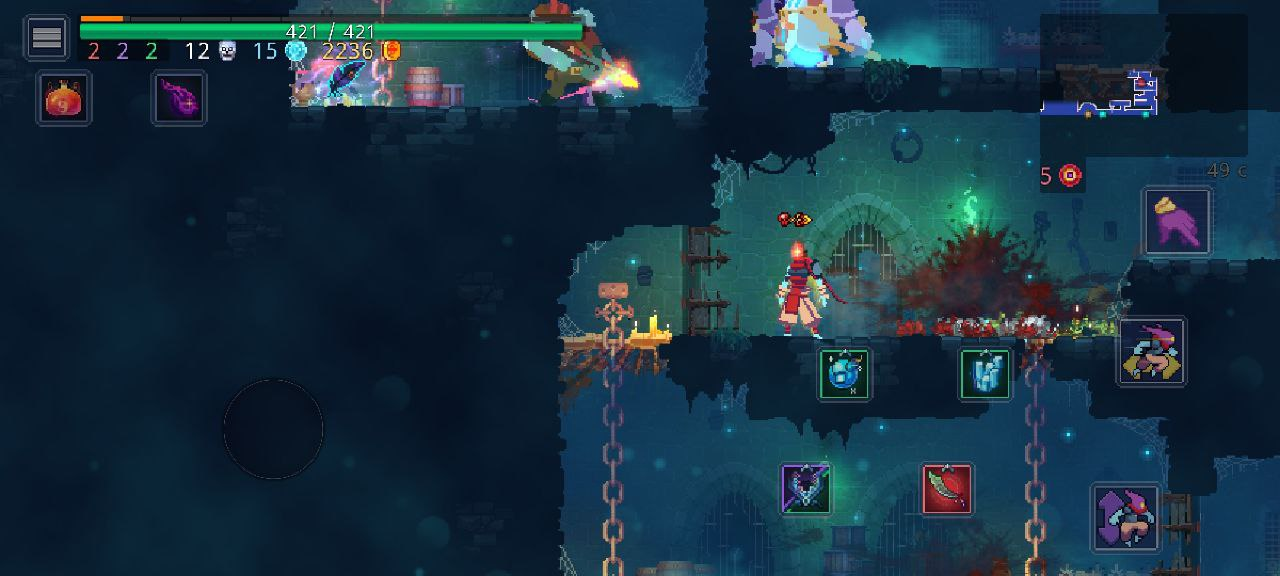
\includegraphics[width=1\textwidth]{primerP}
    \caption{Пример рогалика}
\end{figure}
\begin{figure}[h]
    \centering
    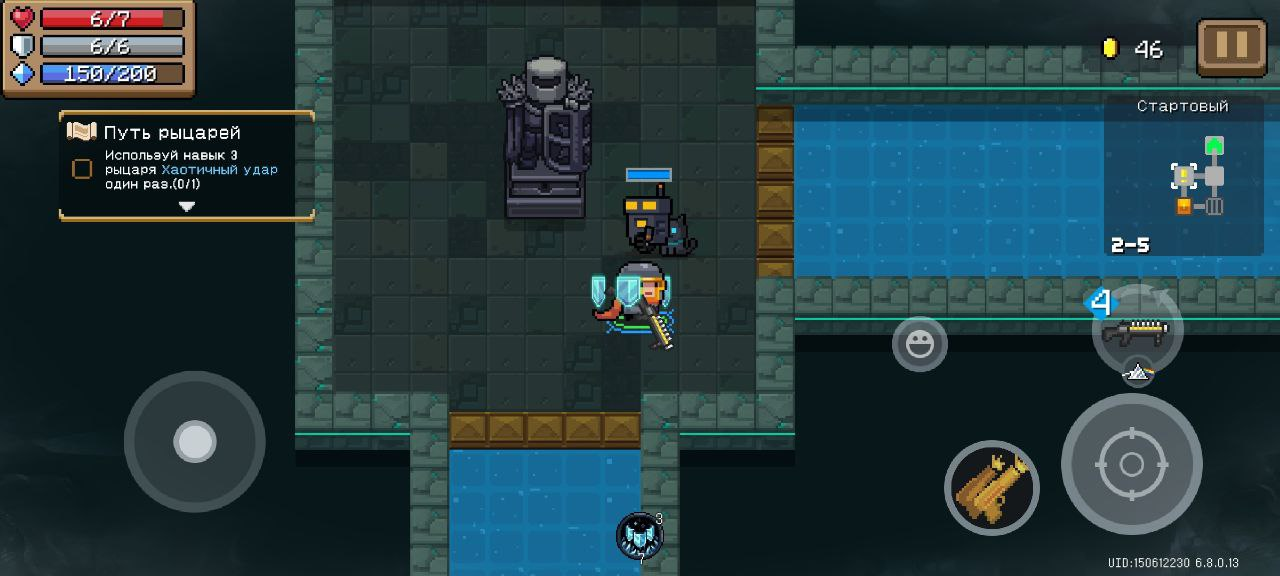
\includegraphics[width=1\textwidth]{primerR}
    \caption{Пример платформера}
\end{figure}
\subsubsection{Ход игры и сюжет}
В начале показывается как главный герой антропоморфное бесформенное существо в мешковатом костюме с капюшоном, после чего появляется гид факелок, который объясняет текущую ситуацию в междугорье и что ему нужно найти и устранить силу поддерживающую проклятье. Дальше игрок двигается вперед по этапам с подсказками гида, основная история локаций и их героев лежит в описании внутриигровых предметов и книгах. Схема прохождения локаций такая: найти первый ключ в первой половине локации, потом найти ключ от подземелья, дальше пройти его и перейти на следующий этап. В финальной локации герои необходимо преодолеть врагов и найти локацию тронного зала, в котором нужно решить  несколько головоломок и (spoiler alert) после чего встретиться с финальным сосредоточением зла - самим собой.
\subsection{Физическая модель}
\subsection{Персонаж игрока}
Для игры roguelike характерным персонажем может быть отважный исследователь подземелий. Аватар игрока может быть представлен в виде смельчака в ржавой броне, с рюкзаком через плечо и факелом в руках, готового идти на поиски сокровищ и приключений. Его лицо может быть скрыто под капюшоном или шлемом, добавляя ауру таинственности.
\subsection{Элементы игры}

\subsection{«Искусственный интеллект»}

\subsection{Многопользовательский режим}


\subsection{Интерфейс пользователя}
\subsubsection{Блок-схема}


\subsubsection{Функциональное описание и управление}


\subsubsection{Объекты интерфейса пользователя}


\subsection{Графика и видео}
\subsubsection{Общее описание}


\subsubsection{Двумерная графика и анимация}


\subsubsection{Трехмерная графика и анимация}


\subsubsection{Анимационные вставки}


\subsection{Звуки и музыка}
\subsubsection{Общее описание}


\subsubsection{Звук и звуковые эффекты}


\subsubsection{Музыка}


\subsection{Описание уровней}
\subsubsection{Общее описание дизайна уровней}


\subsubsection{Диаграмма взаимного расположения уровней}


\subsubsection{График введения новых объектов}


\newpage

\section{Контакты}
Контактная информация для обратной связи.
\end{document}
